\documentclass[10pt]{article}
\usepackage{caption}
\usepackage{amsmath}
\usepackage{array}
\usepackage{url} 
\usepackage{enumerate}
\usepackage[linesnumbered,ruled,vlined]{algorithm2e}
\usepackage{longtable}
\usepackage{multirow} % tables
\usepackage{rotating} % for rotating texts
\usepackage{subfigure}
\usepackage{float}
\usepackage{paralist}
\usepackage{amsfonts}
\pagestyle{empty} % hiding page numbering
\sloppy % for tricky allignments
\usepackage[justification=centering]{caption}
\usepackage{longtable}

\newcolumntype{L}[1]{>{\raggedright\let\newline\\\arraybackslash\hspace{0pt}}m{#1}}
\newcolumntype{C}[1]{>{\centering\let\newline\\\arraybackslash\hspace{0pt}}m{#1}}
\newcolumntype{R}[1]{>{\raggedleft\let\newline\\\arraybackslash\hspace{0pt}}m{#1}}

\DeclareMathOperator*{\argmax}{arg\,max}

\usepackage[a4paper, margin=0.5in]{geometry}
 
\newcommand{\doctitle}{Automatic Image Colorization using Generative Adversarial Networks}


\title{\textbf{\doctitle}\\ \vspace{3mm}
\small {Project Paper of team: Yet Another Layer [YAL]} \\
\small CSci 5561 - Computer Vision } 
\author{Cameron Fabbri, Md Jahidul Islam}

\date{}
\begin{document}
\maketitle

\begin{abstract}
Abstract need to be added Abstract need to be added Abstract need to be added Abstract need to be added 
Abstract need to be added Abstract need to be added Abstract need to be added Abstract need to be added 
Abstract need to be added Abstract need to be added Abstract need to be added Abstract need to be added 
Abstract need to be added Abstract need to be added Abstract need to be added Abstract need to be added 
Abstract need to be added Abstract need to be added Abstract need to be added Abstract need to be added 
  
\end{abstract}

\section{Introduction}\label{sec:intro}
Image colorization \cite{zhang2016colorful, cheng2015deep, bugeau2014variational} refers to colorizing a given gray-scale image so that it appears real. 
A large amount of photographs, videos and movies, mainly antique, lack color; image colorization can provide a modern and vivid view to these images. In addition, surveillance cameras often capture (or store) gray-scale images for convenience. Several underwater inspection and surveillance applications \cite{lu2013underwater, torres2005color} often have to deal with color-less images due to lack of visible light in deep-water. Robust and efficient image colorization techniques can be used in these applications with substantial benefits.   

\begin{figure}[h]
\vspace{-3mm}
\centering
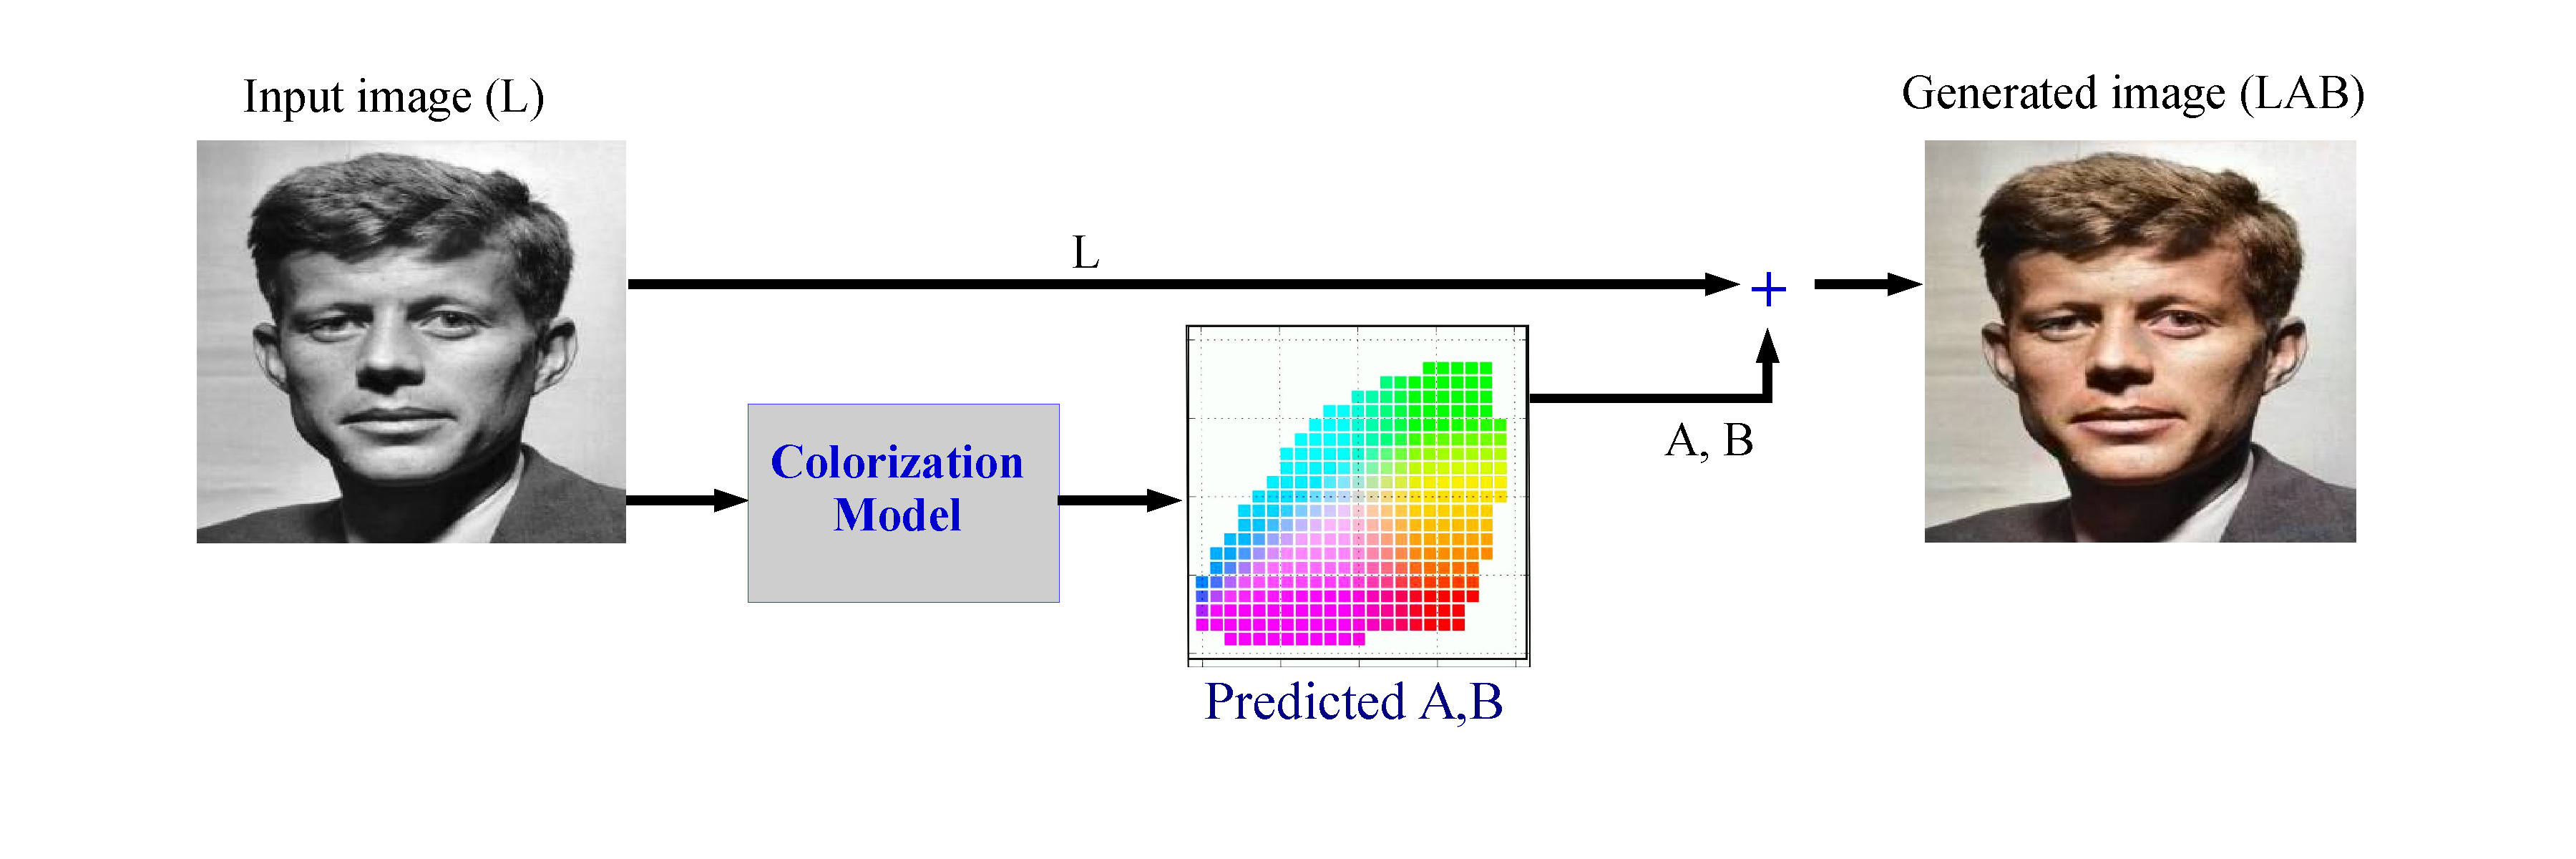
\includegraphics[width=\linewidth]{Figs/6.pdf}
\vspace{-13mm}
\caption{Basic image colorization procedure is shown. LAB color-space is generally used for convenience (\textit{i.e.}, one less unknown dimension); given the lightness channel $L$, task for the colorization model is to predict $A$ and $B$ channels so that the colorized image appears natural. }
\label{fig:col}
\end{figure}  

Colorizing a gray-scale image (\textit{i.e.}, only intensity values are known) is a difficult and ill-posed problem. Computer vision community have approached this problem in different ways over the last few decades \cite{zhang2016colorful, cheng2015deep, bugeau2014variational, charpiat2008automatic, luan2007natural, konushin2006interactive}. Before the advent of deep-learning \cite{lecun2015deep}, researchers have tried many classical techniques \cite{charpiat2008automatic, luan2007natural, konushin2006interactive, levin2004colorization, lagodzinski2008digital} to capture relationships between color components ($RGB$ or $LAB$) and image level features. 
Due to multi-modality and ill-posed nature of the problem, optimization based techniques \cite{levin2004colorization, charpiat2008automatic} and probabilistic models \cite{lagodzinski2008digital} were the only ones that achieved decent colorization performance in few specific applications. 
However, overall performance of these techniques, in general, were still poor due to the high non-linearity and abstract nature of color-feature relationship.  

Recently, deep-learning based image colorization techniques \cite{zhang2016colorful, cheng2015deep, varga2016fully, li2017watergan}, trained over millions of images, have shown significantly better performance over the earlier classical methods. For instance, the current state-of-the-art, `colorful colorization' \cite{zhang2016colorful}, can fool a human observer $32\%$ of the time in a \textit{colorization Turing-test} scenario. \textbf{Additionally,  how use of GANs are likely to improve the performance which why we are going to try?}

\textbf{In this project, we } 
// \textit{need to be added. need to be added. need to be added. need to be added. need to be added. need to be added. need to be added. need to be added.
need to be added. need to be added. need to be added. need to be added. need to be added. need to be added.
need to be added. need to be added. need to be added. need to be added. need to be added.}

\section{Background and Related Work}\label{sec:back}
As mentioned in the previous Section, image colorization is an ill-posed problem due to multi-modality and ambiguity. 
While some natural objects commonly hold the same color (e.g grass is \textit{usually} green), many are left up for interpretation. 
For example, given a gray-scale image of someone wearing a dark colored shirt, 
there is no way of figuring out the true color. 
Instead, the objective is to come up with a colorization that appears real, \textit{i.e.}, natural. 

User-based approaches \cite{levin2004colorization, konushin2006interactive, reinhard2001color, vrhel1992color} were popular for being fast and relatively accurate as user can provide a good prior for the inherent color distribution. However, these methods are not applicable for large scale automatic colorization, which led researchers to adopt optimization and probabilistic approaches \cite{charpiat2008automatic, bugeau2014variational, lagodzinski2008digital}. 
These approaches model a likelihood based color approximation for each pixel given the neighborhood information. 
Few methods introduce additional step for spatial coherency through image based segmentation as well. However, overall colorization performance of these approaches are not very appealing \cite{deshpande2015learning} for general usage in a large scale. This is because the prior distribution of color-space is domain-dependant; for instance, face images, underwater images, outdoor and satellite images, all have different color distributions. Besides, it is difficult to capture the highly non-linear and abstract color-feature relationships without large-scale training. 

In recent times, deep-learning based approaches \cite{zhang2016colorful, cheng2015deep, varga2016fully, li2017watergan} have produced significantly better colorization performance as they can extract highly non-linear spatial relationships if trained over large datasets. 
The convolutional layers learn appropriate filters to produce good feature-space representations from raw images. These feature extraction and filtering is performed over multiple layers 
to capture complex spatial relationships within the image-space, which is useful for image-to-image translation tasks. \textbf{Additionally,  Prospects of GANs GANs .......}

\textbf{In this project, we } 
// \textit{need to be added. need to be added. need to be added. need to be added. need to be added. need to be added. need to be added. need to be added.
need to be added. need to be added. need to be added. need to be added. need to be added. need to be added.
need to be added. need to be added. need to be added. need to be added. need to be added.}  

\section{Generative Approaches}

\section{Adversarial Approaches}

\section{Conclusion}
Abstract need to be added Abstract need to be added Abstract need to be added Abstract need to be added 
Abstract need to be added Abstract need to be added Abstract need to be added Abstract need to be added 
Abstract need to be added Abstract need to be added Abstract need to be added Abstract need to be added 
Abstract need to be added Abstract need to be added Abstract need to be added Abstract need to be added 
Abstract need to be added Abstract need to be added Abstract need to be added Abstract need to be added 

\vspace{1mm}
\bibliographystyle{unsrt}
\footnotesize
\bibliography{cvbibs}

\end{document}
